\documentclass[spanish,notitlepage,letterpaper,11pt]{article} % para artículos en español

\usepackage[utf8]{inputenc} % Acepta caracteres en español
\usepackage[T1]{fontenc} % font encoding
\usepackage[spanish,es-tabla]{babel} % silabea palabras en español
\usepackage{amsmath}
\usepackage{amsfonts}
\usepackage{amssymb}
\usepackage[colorlinks=true,urlcolor=blue,linkcolor=blue]{hyperref} % navega por el doc
\usepackage{graphicx}
\usepackage{geometry} % See geometry.pdf to learn the layout options.
\usepackage{fancyhdr} % encabezados y pies de pg


\voffset = -0.25in 
\textheight = 8.0in 
\textwidth = 6.5in
\oddsidemargin = 0.in
\headheight = 20pt 
\headwidth = 6.5in

%%%%%%%%%%%%%%%%%%%%%%%%%%%%%%%%%%%%%%%%%%%%%%%%%%%%%%%%%%
%% NO TOCAR NADA DE LO QUE ESTA ARRIBA DE ESTA ZONA AZUL 
%%%%%%%%%%%%%%%%%%%%%%%%%%%%%%%%%%%%%%%%%%%%%%%%%%%%%%%%%%

\pagestyle{fancy} 
\chead{\bfseries Aquí va el Título de la practica} 
\lhead{\begin{picture}(0,0) \put(0,0){
\includegraphics[width=30mm]{figuras/logouis}} \end{picture}} 
\rhead{20/01/2024} 
\lfoot{  } 
\cfoot{Universidad Industrial de Santander} 
\rfoot{\thepage} 


\begin{document}
\begin{figure}
{
\includegraphics[width=40mm]{figuras/logouis}} 
\end{figure}
\title{\bf Aquí va el Título de la practica 1}
\author{
\textbf{Pedro Perez}\thanks{\texttt{pperez@uis.edu.co}} \\
\textit{Escuela de F\'isica, Universidad Industrial de Santander,}\\ 
\textit{Bucaramanga 680002, Colombia}, \\
\textbf{Menchi Ibarra}\thanks{\texttt{imenchi@uis.edu.co}} \\
\textit{Escuela de Q\'imica, Universidad Industrial de Santander},\\ 
\textit{Bucaramanga 680002, Colombia},  y \\
\textbf{Firulais Sánchez}\thanks{\texttt{firus@gmail.com}} \\
\textit{Escuela de Biología, Universidad Industrial de Santander,  }\\ 
\textit{Bucaramanga 680002, Colombia}. 
}
\date{Versión 1.0 - \today}
\maketitle
\tableofcontents
\newpage
\begin{abstract}
El resumen debe ser suficiente para que uno no se lea el documento y tenga la idea completa de qué se hizo y cuáles fueron los resultados. Tiene que ser un ``articulito'' que indique en frases telegráficas: la importancia de problema a estudiar ({\it Introducción}), cómo se estudió ({\it Metodología}), cuáles fueron los resultados ({\it Resultados}) y cuál es la importancia de los  resultados ({\it Conclusiones}). Toda la información importante y trascendente del documento debe estar aquí. 

Escribir un buen resumen es clave porque uno anuncia lo que viene. Cuando postulamos una presentación a un congreso enviamos un resumen y allí quizá nos ganamos una charla o nos conformamos con un póster. 

El resumen es lo último que se redacta y contiene frases y oraciones que luego el lector se encontrará en el artículo. La intención es que esas frases, esas ideas la re-encuentre el lector en texto 

Típicamente debe tener una extensión entre 150 a 250 palabras. No tiene que ser un párrafo monolítico, porque se contabilizan las palabras. Entonces uno puede jugar los los párrafos para fijar las ideas. 

En estos enlaces pueden consultar algunos buenos consejos para la redacción de resúmenes:  
\begin{itemize}
    \item \url{https://breathe.ersjournals.com/content/10/3/265}, 
    \item \url{http://amj.amegroups.com/article/view/4965/html}, 
    \item \url{https://chemistrycommunity.nature.com/posts/43071-how-to-write-an-abstract}
    \item \url{https://mitcommlab.mit.edu/broad/commkit/journal-article-abstract/ }
\end{itemize}

\end{abstract}

\section{Introducción}
Es el ¿Qué? del artículo. Aquí debe ir la descripción del problema, su importancia, sus antecedentes. Seguidamente, la justificación de este reporte, por qué se hace la investigación o reporta un caso, como se enmarca en los antecedentes y cuál es su importancia. Es importante, en la introducción resaltar los aportes de este trabajo con los antecedentes que los precedieron. Los acrónimos deben ser explicitados la primera vez que aparezcan.

La presentación de la introducción va de lo general a lo particular. Se presenta primero el contexto (el área temática) dónde se enmarca el artículo y su importancia. Luego sigue el problema concreto que motiva este trabajo y, finalmente, lo puntual de la contribución que abordará el artículo. 

La construcción de la introducción es un cono invertido, de lo general a lo particular. En la introducción se muestra el manejo y la actualidad de la bibliografía del tema, general y particular.  La importancia de contribución concreta. Es importante anunciar lo que viene sin dar detalles al desenlace. Hay que buscar que el lector quede con inquietudes e incógnitas que lo lleven a leerse el artículo. 

Hay colegas que tienden a redactar la introducción al principio y esa redacción les aclara las ideas. Hay grupos de investigación que tienen miembros especializados en hacer la introducción. Son gente que tiene una visión amplia del tema y maneja la bibliografía.  En mi caso es los penúltimo que redacto: último el resumen y antes del resumen la introducción. 

En estos dos enlaces hay recomendaciones concretas para redactar una buena introducción
\begin{itemize}
    \item \url{http://amj.amegroups.com/article/view/4738/html}
    \item \url{https://mitcommlab.mit.edu/broad/commkit/journal-article-introduction} 
\end{itemize}

En este otro enlace: \url{http://amj.amegroups.com/article/view/4983/html} se detalla un gran conjunto de recomendaciones generales para redactar un artículo.

Esta sección se debe finalizar con una descripción de lo que viene. Qué contienen cada una de las secciones. En la Sección \ref{Metodologia} discutimos la metodología empleada, mientras que en la Sección \ref{Resultados} se presentan los resultados. Finalizamos el artículo con las conclusiones en la Sección \ref{Conclusiones}.


\section{Metodología}
\label{Metodologia}

Es el ¿cómo? del artículo. En esta sección se cuenta cómo se montó el experimento o cómo se planteó la simulación. La metodología experimental o teórica utilizada, sus detalles, haciendo referencia a los antecedentes que justifican las técnicas (experimentales o computacionales) empleadas. Cuáles herramientas (o técnicas) se utilizaron, por qué se utilizaron y cuáles son sus ventajas y las desventajas respecto a las existentes. 

Esta sección tiene que garantizar la reproducibilidad del experimento o el cálculo, por lo tanto tendrán que adjuntar las mediciones y/o los archivos de datos resultados de las simulaciones. 

Algunas recomendaciones generales para redactar la metodología la pueden encontrar en este enlace: \url{https://mitcommlab.mit.edu/broad/commkit/journal-article-methods/}

\section*{Sobre las tablas, figuras, listas y ecuaciones}

A continuación se muestra, a modo de información para los que estamos aprendiendo a escribir en \LaTeX,  una serie de recomendaciones y comentarios para introducir: tablas, figuras, listas y ecuaciones matemáticas. 

\subsection*{Tablas}
Las tablas forman parte de la narración y deben estar presentadas como un complemento al texto. Las Tablas deben ser lo más autocontenidas posibles. Sus títulos y  leyendas deben ser suficiente para explicar su contenido. Las leyendas de tablas y figuras deben ser más que una simple descripción. Deben generar una reflexión una conclusión al presentar la tabla o figura.

Obviamente, las tablas tienen que estar referidas desde el texto (ver Tabla \ref{Tabla1}). Si no se hace referencia a una tabla en particular, ésta se considera inútil para el artículo y debe ser suprimida.
\begin{table}[!ht]
  \centering
  \caption{Las leyendas de las tablas se diferencia de las de la figuras porque van arriba. Deben explicar el contenido de las tablas. No ser meras descripciones de lo que se ve en las tablas. Deben generar reflexión respecto a lo que se quiere evidenciar en la tabla }  
  \vspace{0.3cm}
\begin{tabular}{|l|c|r|} 
\hline
% after \\ : \hline or \cline{col1-col2} \cline{col3-col4} ... este campo se usa para multicolumna
  Evento 1 & Evento 2  & Evento 3  \\ \hline \hline
  Justificado Izquierdo & centrado & Justificado derecho \\\hline  
  A & B  & C \\ \hline 
  1 & 2 & 3 \\ \hline 
 \vdots & \vdots & \vdots \\  \hline \hline
\end{tabular}   
  \label{Tabla1}
\end{table}

Existen varios generadores de tablas en linea, por ejemplo: \url{https://www.tablesgenerator.com}. 

En la Tabla \ref{Tabla2} mostramos otro ejemplo de construcción para tablas en \LaTeX

\begin{table}[!ht]
\centering
\caption{Velocidad de carrera sobre 200$ \mathrm{~m}$ y distancia de salto de longitud  de un grupo de personas seleccionadas al azar.\\
Nota: El participante 4 no pudo realizar el salto de longitud  por razones médicas.}
  \vspace{0.3cm}
\begin{tabular}{ccc}
\hline Participante & Velocidad $\left(\mathrm{ms}^{-1}\right)$ & Distancia $(\mathrm{m})$ \\ \hline \hline 
1 & 10.53 & 2.38 \\
2 & 11.16 & 1.83 \\
3 &  9.54  & 2.04 \\
4 & 15.77 & NA \\
5 & 12.82 & 1.74 \\
& & \\
Total & 59.82 & 7.99 \\
Promedio & 11.964 & 1.997 \\
\hline
\end{tabular}
\label{Tabla2}
\end{table}


\subsection*{Figuras}
Al igual que las Tablas, las figuras forman parte de la narración. Deben ser lo mas autocontenidas posibles. Sus títulos y  leyendas deben ser suficiente para explicar su contenido y el mensaje que se quiere dejar con la figura. 
\begin{figure}[!ht]
\begin{center}
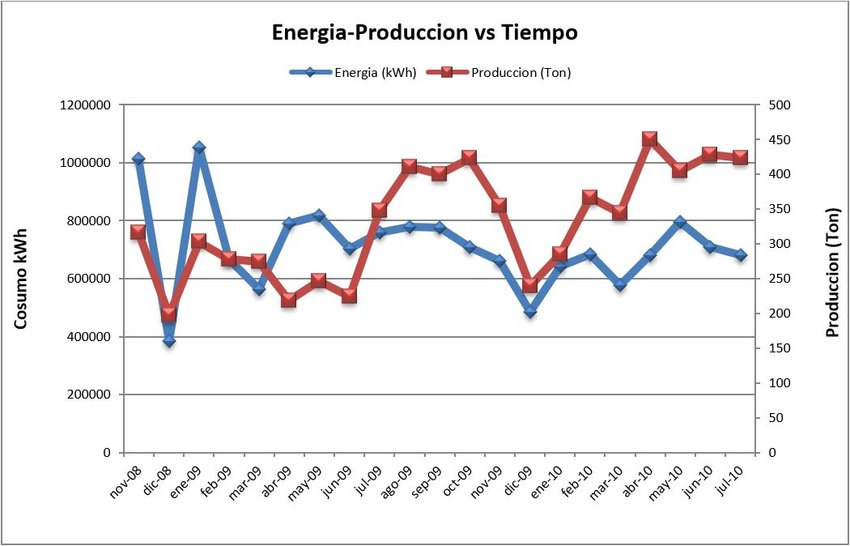
\includegraphics[width=3.6in]{figuras/fig01.png}
\caption{Esta figura incorpora una imagen. Las Figuras deben ser lo mas autocontenidas posibles. Sus títulos y  leyendas deben ser suficiente para explicar su contenido. No deben ser meras descripciones. Si las figuras no son construidas por el autor, se debe tener cuidado de verificar la posible licencia de uso.}
\label{Figura1}
\end{center}
\end{figure}

Las figuras son claves para la presentación de los resultados. Muchas veces los lectores expertos en un tema, luego del resumen van a las figuras. Si los resultados que éstas presentan les llaman la atención, comienzan a revisar con mas cuidado el artículo. Por ello, todo el tiempo que le dediquen a presentar buenas y claras figuras rendirán beneficios a la calidad e impacto del artículo 

Las figuras deben ser referidas desde el texto (ver Figura \ref{Figura1}). Otra vez, si no se hace referencia a una figura en particular, ésta se considera inútil para el artículo y debe ser suprimida.

Hay que tener cuidado con las figuras que uno incluye en su reporte. Si las obtenemos de ``internet'' debemos estar seguros que la podemos reutilizar. La políticas y licencias de acceso abierto permiten reutilizar textos y gráficos. El acceso abierto (OA) es un conjunto de principios y prácticas a través de las cuales los resultados de la investigación se distribuyen en línea, sin costo ni barreras de acceso\footnote{Para mayores detalles pueden consultar:  \url{https://en.wikipedia.org/wiki/Open_access}}.


\subsection*{Elaboración de listas}
Las lista pueden ser numeradas
\begin{enumerate}
\item naranjas
\item papayas
\end{enumerate}

o no numerada
\begin{itemize}
\item naranjas
\item papayas
\end{itemize}

\subsection*{Escritura de ecuaciones matemáticas}
Esto es el fuerte de la escritura en \LaTeX{}, como veremos, se puede escribir ecuaciones matemáticas en alta calidad tipográfica. Veamos algunos ejemplos:

Sean $X_1, X_2, \ldots, X_n$ una sucesión  de variables aleatorias independientes e idénticamente distribuidas con $\text{Var}[X_i] = \sigma^2 < \infty$, y sea
$$
S_n = \frac{X_1 + X_2 + \cdots + X_n}{n} = \frac{1}{n}\sum_{i}^{n} X_i
$$

También se puede ir escribiendo las ecuaciones para que vayan apareciendo numeradas:
\begin{equation}
  S_n = \frac{X_1 + X_2 + \cdots + X_n}{n} = \frac{1}{n}\sum_{i}^{n} X_i 
  \label{Suman}
\end{equation}

Para familiarizarnos con las formulas matemáticas en \LaTeX{} podemos usar el siguiente generador:  \url{https://latex.codecogs.com/eqneditor/editor.php?lang=es-es}. 

Obviamente se puede citar las ecuaciones.  La ecuación (\ref{Suman}) la citaremos cuando necesitemos hacer referencia a ella.


\section{El experimento y los resultados}
\label{Resultados}
¿Qué se midió o se simuló? ¿cuáles fueron las condiciones de medición o las de simulación, los códigos o sistemas computacionales? ¿que representan esas medidas o resultados de simulaciones? ¿cuáles son las limitaciones de la medida por las restricciones que impone la técnica y las herramientas? Todo esto debe quedar registrado de manera que permita que esos resultados sean reproducibles por otras personas.

Las figuras presentan los resultados, dan la la oportunidad de examinar directamente los datos y sacar sus propias conclusiones. En la sección de resultados los autores guían esa interpretación explicando la lógica experimental y/o computacional, destacando las características importantes de los datos y exponiendo las conclusiones.

Esta sección anuncia lo que se discutirán a fondo en la sección de conclusiones.

En este enlace se exponen con detalle algunas de las estrategias que se pueden seguir en la construcción de la sección de resultados:\\ 
 \url{https://mitcommlab.mit.edu/broad/commkit/journal-article-results}. 


\section{Conclusiones y recomendaciones}
\label{Conclusiones}
El primer párrafo de las conclusiones debe mostrar cuál es el aporte del trabajo. Cuál es su importancia y trascendencia. 

La estructura de las conclusiones es invertida a la de la introducción. Comienza explicitando/enumerando los principales resultados. Luego sigue una interpretación de esos resultados y finaliza con la trascendencia de los resultados.  

Quizá la mejor recomendación es consultar el libro de Umberto Eco, {\it Cómo hacer una Tesis Doctoral} \cite{Eco1986} 

Otra posible fuente de información puede ser el libro \textit{A guide to Effective Publishing in Astronomy} \cite{BertoutBiemesderferHenri2012} donde además aparece reseñado todo el proceso de publicación en Astronomía\footnote{\url{https://astro.mff.cuni.cz/vyuka/AST031/guide.pdf}}.

Los siguientes enlaces registran muy buenas recomendaciones para redactar la sección de conclusiones 
\begin{itemize}
    \item \url{https://www.academia.edu/11983516/Slightly_updated_version_of_the_How_to_write_a_conclusion_ppt}
    \item \url{http://amj.amegroups.com/article/view/4955/html }
    \item \url{https://mitcommlab.mit.edu/broad/commkit/journal-article-discussion/ }
\end{itemize}


\section*{Nota sobre el uso de los apéndices}

La decisión de incluir apéndices en un informe o artículo científico depende de varios factores y puede variar según el tipo de trabajo y las pautas editoriales de la revista o conferencia. En \LaTeX{} se deben agregar de la manera siguiente:

\appendix
\section{Aquí va el título del apéndice}
Los apéndices en un informe o artículo científico tienen varios propósitos. Aquí se describen algunas de las razones comunes para incluir apéndices en un documento:
\begin{itemize}
\item Detalles Técnicos Adicionales:

Los apéndices pueden contener información técnica adicional que complementa el contenido principal del documento. Esto puede incluir detalles sobre métodos, cálculos, algoritmos, o cualquier material que sea importante para la comprensión del lector pero que sería demasiado extenso o detallado para incluir en el cuerpo principal del artículo.

\item Datos y Resultados Completos:

Si el artículo se basa en un conjunto de datos extenso o en resultados adicionales que son relevantes para la comprensión completa del trabajo, esos datos o resultados completos pueden ser colocados en un apéndice.

\item Material Suplementario:

Información suplementaria, como gráficos adicionales, tablas extensas, fotografías, o cualquier otro material que complemente el artículo, puede colocarse en los apéndices.

\item Documentos Relacionados:

A veces, se incluyen documentos adicionales relevantes, como cuestionarios, encuestas, protocolos de prueba, o cualquier otro material relacionado.

\item Código Fuente o Algoritmos:

Si el trabajo implica el desarrollo de algoritmos o software, el código fuente o descripciones detalladas de los algoritmos pueden ubicarse en los apéndices.

\item Información No Esencial para la Narrativa Principal:

Información que no es esencial para la narrativa principal del artículo pero que puede ser de interés para algunos lectores puede ubicarse en los apéndices. Esto ayuda a mantener el enfoque del cuerpo principal del artículo en los resultados y conclusiones clave.
\end{itemize}


\section{Aquí va el título del apéndice}
Al usar apéndices, es importante que estos complementen y enriquezcan el contenido del artículo principal, proporcionando detalles adicionales o material de soporte sin abrumar al lector. La clave es equilibrar la cantidad de información en el cuerpo principal del artículo y en los apéndices para ofrecer una presentación clara y efectiva del trabajo.

Los apéndices deben mejorar la comprensión del lector y no sobrecargar el documento principal. Antes de decidir incluir apéndices, considera la audiencia a la que te diriges, la relevancia del material adicional y las pautas específicas de formato de la revista o conferencia a la que planeas enviar tu trabajo. Siempre verifica las recomendaciones y normativas de la publicación a la que estás enviando tu artículo.

\section*{Sobre la bibliografía}

Aquí deben ir las referencias citadas \cite{Narasimhan1993, Chandra1950} y cuando corresponda, los {\bf url} que se consideren necesarios y que hayan sido citadas en el texto del documento. Como se puede ver, es fácil  hacer las citas pues se escribe 
\begin{verbatim}\cite{Demianski1985}\end{verbatim}

Entre llaves ponemos la etiqueta que hemos escogido para llamar la cita bibliográfica, lo que resulta en la cita con su enlace \cite{Demianski1985}

Es mucho más fácil utilizar \texttt{Bibtex}, que es un mecanismo para citar referencias siguiendo los patrones internacionales. Si no se hace uso de \texttt{Bibtex} se tiene que tener cuidado de citar de la forma que lo requiera la publicación. Si no hay recomendaciones de los editores, lo mejor es apegarse a algún estilo estándar y civilizado de presentar la bibliografía 

Hay bastante información disponible:\\
\url{https://www.overleaf.com/learn/latex/Bibliography_management_in_LaTeX}. 

Por último, es muy importante que las citas tengan  una  referencia en el texto, es decir, no se debe agregar citas sin que en el texto del artículo se hallan mencionado, no puede haber referencias solas. 


\begin{thebibliography}{}

\bibitem{Eco1986} Eco, U. \\
\textit{C{\'o}mo se hace una tesis}. Barcelona, Editorial Gedisa (1993)

\bibitem{BertoutBiemesderferHenri2012} Bertout, C. and Biemesderfer, C. and Henri, A.  \\
\textit{A guide to Effective Publishing in Astronomy}. EDP Science (2012) \\
\url{https://astro.mff.cuni.cz/vyuka/AST031/guide.pdf}

\bibitem{Narasimhan1993}Narasimhan M. N. L.  \\
\textit{Principles of Continuum Mechanics}. John Willey, New York (1993)

\bibitem{Chandra1950}Chandrasekhar S.  \\
\textit{Radiative Transfer}. Oxford, Oxford University Press (1950)

\bibitem{Demianski1985}Demia\'{n}ski M. \\
\textit{Relativistic Astrophysics}, in International Series in Natural Philosophy, 
Vol 110, Edited by  \textit{D. Ter Haar}. Pergamon Press, Oxford (1985)

\end{thebibliography}


\end{document}  